\section{Empirical Dust Attenuation Modeling} \label{sec:dem}
In this section we present the Empirical Dust Attenuation (\eda) model, a
flexible prescription for applying attenuation curves to galaxy populations 
that allows us to incorporate intrinsic variations in dust attenuation as well
as correlation to physical galaxy properties. Later, we demonstrate that we can
accurately reproduce SDSS observations with the \eda~and use it to test galaxy
formation models and shed light on dust in galaxies. 

We define the dust attenuation curve, $A(\lambda)$, as 
\begin{equation} 
    F_o (\lambda) = F_i (\lambda) 10^{-0.4 A(\lambda)}
\end{equation}
where $F_o$ is the observed flux and $F_i$ is the intrinsic flux. We normalize
the attenuation at the $V$ band, 
\begin{equation} 
    A(\lambda) = A_V \frac{k(\lambda)}{k_V}
\end{equation}
so that $A_V$ determines the amplitude of the attenuation, while $k(\lambda)$
determines the wavelength dependence. 

To determine $A(\lambda)$ for each galaxy, we first assign $A_V$ using the slab
model from~\cite{somerville1999, somerville2012}. In the slab model, $A_V$ is
calculated from the inclination of the galaxy, $i$, and its optical depth, $\tau_V$: 
\begin{equation} \label{eq:slab}
    A_V = -2.5 \log \left[ \frac{1 - e^{-\tau_V\,\sec i}}{\tau_V\,\sec i} \right].
\end{equation}
For all of our galaxies, we uniformly sample $i$. We then include the
correlation between $A_V$ and galaxy properties ($M_*$ and $\sfr$), found
in both observations and simulations~\citep[\eg][]{narayanan2018, salim2020},
in $\tau_V$. We use $\tau_V$ with a simple and flexible linear $M_*$ and $\sfr$ 
dependence:
\begin{equation} \label{eq:tauv}
    \tau_V(M_*, \sfr) = \mtaum \log \left(\frac{M_*}{10^{10} M_\odot}\right) + \mtaus \log\,\sfr + c_\tau.
\end{equation}
$\mtaum$ quantifies the $M_*$ dependence, $\mtaus$ quantifies the $\sfr$
dependence, and $c_\tau$ quantifies the overall amplitude. Since $\tau_V$ is
optical depth, we impose a $\tau_V \ge 0$ limit. We note that the slab model 
is a naive approximation. In reality, $A_V$ for a galaxy will depend on complexities 
of its star-to-dust geometry, variations in the extinction curves, and other
properties beyond just inclination and $\tau_V$. The purpose of the \eda,
however, is not to accurately model dust attenuation for individual galaxies,
but rather to accurately model the distribution of dust attenuation for galaxy
populations. In this sense, the slab model qualitatively reproduces the
correlation between $A_V$ and $i$ found in the literature: edge-on galaxies
have higher $A_V$ than face-on galaxies~\citep[\eg][]{conroy2010, wild2011,
battisti2017, salim2020}. More
importantly, the $A_V$ distribution, $p(A_V)$, produced using the slab model with
uniformly sampled inclinations closely matches the $p(A_V)$ of our SDSS sample
(Figure~\ref{fig:av_dist}). Also, replacing the slab model with a more flexible
prescription for sampling $A_V$ does not significant
impact our analysis (Appendix~\ref{sec:nonslab}). We therefore conclude that
the slab model is a sufficiently flexible empirical prescription for sampling
$A_V$. 

For the wavelength dependence of the attenuation curve, $k(\lambda)$, we
use the \cite{noll2009} parameterization: 
\begin{equation} \label{eq:noll}
    k(\lambda) = \left(k_{\rm Cal}(\lambda) + D(\lambda)\right) \left(
    \frac{\lambda}{\lambda_V} \right)^\delta.
\end{equation}
Here $k_{\rm Cal}(\lambda)$ is the \cite{calzetti2001} curve: 
\[
    k_{\rm Cal}(\lambda) = 
    \begin{cases} 
        2.659 (-1.857 + 1.040/\lambda) + R_V, & 6300 \AA \le \lambda \le
        22000 \AA \\ 
        2.659 (-2.156 + 1.509/\lambda - 0.198/\lambda^2 + 0.011/\lambda^3) +
        R_V & 1200 \AA \le \lambda \le 6300 \AA
    \end{cases}
\]
where $\lambda_V = 5500 \AA$ is the $V$ band wavelength. $\delta$ is the slope
offset of the attenuation curve from $k_{\rm Cal}$. Since $\delta$ correlates 
with galaxy properties~\citep[\eg][]{leja2017, salim2018},
we parameterize $\delta$ with a similar $M_*$ and $\sfr$ dependence as
$\tau_V$:  
\begin{align} \label{eq:delta}
    \delta(M_*, \sfr) &= \mdeltam \log \left(\frac{M_*}{10^{10}
    M_\odot}\right) + \mdeltas \log\,\sfr + c_\delta 
\end{align}
% Although a number of works have found correlation between the attenuation
% curve slope and inclination~\citep{wild2011, chevallard2013, battisti2017b},
% \cite{salim2020}, most recently, found that the driver of this trend is the
% relationship between $A_V$ and slope. We therefore do not include an
% inclination dependence in $\delta$. 
$D(\lambda)$ in Eq.~\ref{eq:noll} is the UV dust bump, which we parameter using
the standard Lorentzian-like Drude profile:
\begin{equation}
    D(\lambda) = \frac{E_b(\lambda \Delta \lambda)^2}{(\lambda^2 -
    \lambda_0^2)^2 + (\lambda \Delta \lambda)^2}
\end{equation}
where $\lambda_0$, $\Delta \lambda$, and $E_b$ are the central wavelength,
FWHM, and strength of the bump, respectively. We assume fixed $\lambda_0 = 2175
\AA$ and $\Delta \lambda = 350\AA$. \cite{kriek2013} and \cite{tress2018} find
that $E_b$ correlates with the $\delta$ for star-forming galaxies $z\sim2$.
\cite{narayanan2018} confirmed this dependence in simulations. In our \eda~
model, we assume a fixed relation between $E_B$ and $\delta$ from \cite{kriek2013}: 
$E_b = -1.9~\delta + 0.85$. Allowing the slope and amplitude of the $E_B$ and
$\delta$ relation to vary, does {\em not} impact our results.
In Table~\ref{tab:free_param}, we list and describe all of the free parameters
in the \eda. 

%Next, to attenuate the galaxy SEDs, we apply $A(\lambda)$ we separately to the
%star light and nebular emssion: 
%\begin{equation} \label{eq:full_atten}
%    F_o (\lambda) = F^{\rm star}_i (\lambda) 10^{-0.4 A(\lambda)} + F^{\rm
%    neb}_i (\lambda) 10^{-0.4 A_{\rm neb}(\lambda)}.
%\end{equation}
%We parameterize
%\begin{equation}
%    A_{\rm neb}(\lambda) = f_{\rm neb}  A(\lambda) 
%\end{equation} 
%and allow $f_{\rm neb}$ to vary freely. 

$\sfr$ of galaxies are used to calculate $\tau_V$ and $\delta$ in
Eqs.~\ref{eq:tauv} and~\ref{eq:delta}. Due to mass and temporal resolutions,
some galaxies in the simulations have $\sfr=0$ --- \ie~an unmeasurably low
SFR~\citep{hahn2019c}. Eqs.~\ref{eq:tauv} and~\ref{eq:delta} cannot be used to
derive $\tau_V$ and $\delta$ for these galaxies. Since $\sfr=0$ galaxies do
not account for a large fraction of our simulated galaxies, we directly sample 
their observables ($G, R, NUV$, and $FUV$) from the distribution of observables
for SDSS quiescent galaxies. This way, we ensure that the attenuation of $\sfr=0$ 
galaxies does not impact the rest of the \eda~parameters. In Appendix~\ref{sec:res}, 
we discuss the resolution effects in more detail and demonstrate that our results
are \emph{not} impacted by other prescriptions for attenuating $\sfr=0$ galaxies.

To apply the \eda~to a simulated galaxy population in practice, we begin by
uniformly sample inclinations, $i$, and assign them to each galaxy. Then for a
given set of \eda~parameter values, $\tau_V$, and $\delta$ are calculated for
each galaxy using its $i$, $M_*$, and $\sfr$. From $\tau_V$ and $\delta$, we
determine $A_V$ and $k(\lambda)$, which together gives $A(\lambda)$ for each of
the galaxies.  Afterwards, we attenuate the galaxy SEDs using Eq.~\ref{eq:full_atten} and use 
the attenuated SEDs to calculate the observables: $G, R, NUV$, and $FUV$
absolute magnitudes. In Figure~\ref{fig:dem_av}, we present the \eda~ 
$A(\lambda)$
for galaxies with different $\sfr$ and $M_*$: 
star-forming ($\sfr=10^{0.5}M_\odot/yr$) with low mass ($10^{10}M_\odot$;
blue), with high mass ($10^{11}M_\odot$; green) and quiescent
($\sfr=10^{-2}M_\odot/yr$) with low mass ($10^{10}M_\odot$; orange), with high
mass ($10^{11}M_\odot$; red). All galaxies are edge-on (\ie~$i=0$) and we use
$\{\mtaum, \mtaus, c_\tau, \mdeltam, \mdeltas,
c_\delta\} = \{2., -2., 2., -0.1, -0.1, -0.2\}$, which were arbitrarily chosen
within the prior range listed in Table~\ref{tab:free_param}. For comparison, we 
include the \cite{calzetti2001} attenuation curve. The \eda~we describe in this 
section provides a flexible model for assigning a wide range of dust attenuation 
to galaxies based on their physical properties. 


Next, we measure the observables by convolving the SEDs by
transmission curves of the GALEX $FUV$, GALEX $NUV$, SDSS $g$, and SDSS $r$
broadband filters. Lastly, we add realistic noise to $M_r$, $\gr$, and $\fnuv$. 
We sample the noise from normal distributions, where the standard deviations 
are drawn from $\chi^2$ fits to the the observed uncertainty distributions from 
NASA-Sloan Atlas.



\begin{figure}
\begin{center}
    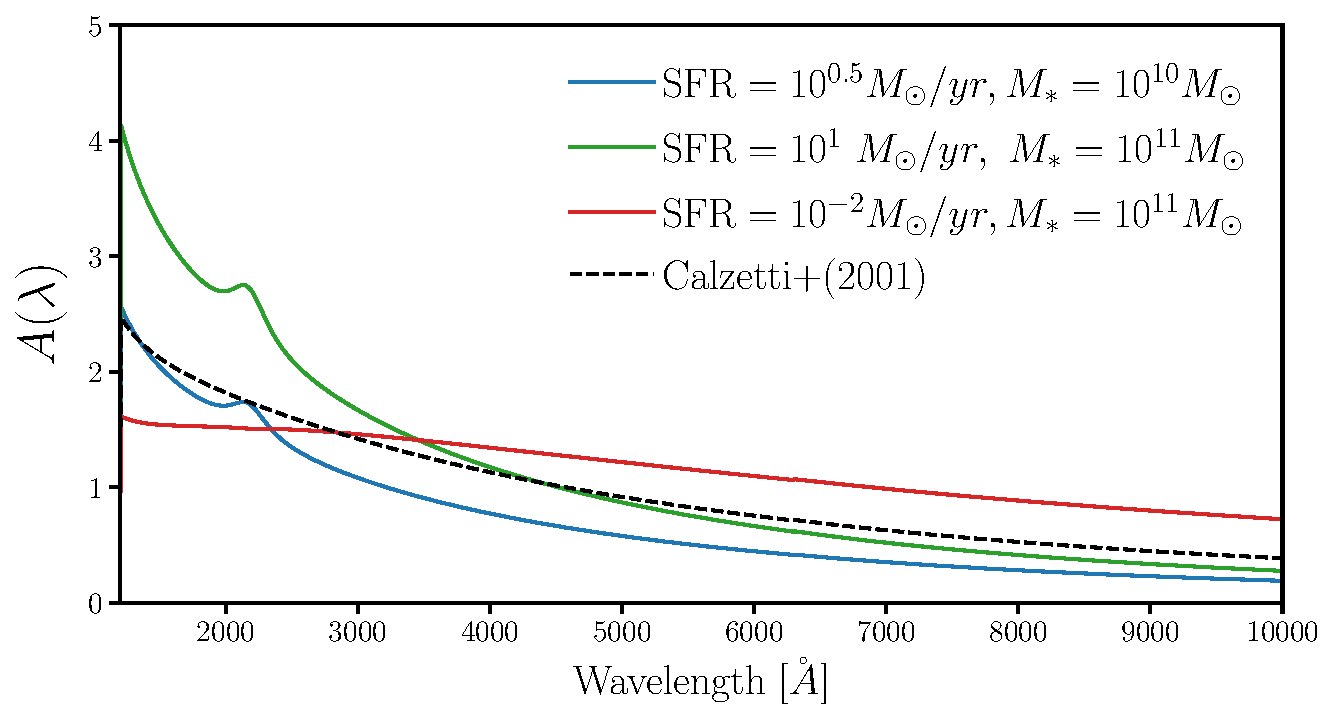
\includegraphics[width=0.6\textwidth]{figs/dems.pdf}
    \caption{\label{fig:dem_av}
    Attenuation curves, $A(\lambda)$, of our Empircial Dust Attenuation (\eda)
    model for galaxies with different $\sfr$ and $M_*$. We include $A(\lambda)$ for 
    star-forming ($\sfr=10^{0.5}M_\odot/yr$) low mass galaxy ($10^{10}M_\odot$;
    blue), high mass galaxy ($10^{11}M_\odot$; green) and quiescent
    ($\sfr=10^{-2}M_\odot/yr$) low mass galaxy ($10^{10}M_\odot$; orange), 
    high mass galaxy ($10^{11}M_\odot$; red). All galaxies are edge-on
    (\ie~$i=0$) and we use \eda~parameter values $\{\mtaum, \mtaus, c_\tau, \mdeltam, \mdeltas,
    c_\delta\} = \{2., -2., 2., -0.1, -0.1, -0.2\}$ near the center of our prior range
    (Table~\ref{tab:free_param}). For comparison, we include the \cite{calzetti2001} 
    attenuation curve. In the \eda, the amplitude, slope, and UV dust bump of
    $A(\lambda)$ depend on $M_*$, and $\sfr$ (Eqs.~\ref{eq:tauv}
    and~\ref{eq:delta}). {\em The \eda~provides a flexible model for
    assigning dust attenuation to galaxies based on their physical properties}.
    } 
\end{center}
\end{figure}


%%%%%%%%%%%%%%%%%%%%%%%%%%%%%%%%%%%%%%%%%%
% table of free parameters
%%%%%%%%%%%%%%%%%%%%%%%%%%%%%%%%%%%%%%%%%%
\begin{table}
    \caption{Parameters of the Dust Empirical Model}
    \begin{center}
        \begin{tabular}{ccc} \toprule
            Parameter & Definition & prior\\[3pt] \hline\hline
            %\multicolumn{3}{c}{DEM with slab model}\\ \hline
            $\mtaum$ & Slope of the optical depth, $\tau_V$, $\log M_*$ dependence & flat $[-5., 5.]$\\
            $\mtaus$ & Slope of the optical depth, $\tau_V$, $\log {\rm SFR}$ dependence & flat $[-5., 5.]$\\
            $c_{\tau}$ & amplitude of the optical depth, $\tau_V$ & flat $[0., 6.]$\\
            %\hline
            %\multicolumn{3}{c}{DEM with $\mathcal{N}_T$ model}\\ \hline
            %$m_{\mu,1}$ & Slope of the $\log M_*$ dependence of optical depth,
            %$\tau_V$ & flat $[-5., 5.]$\\
            %$m_{\mu,2}$ & Slope of the $\log {\rm SFR}$ dependence of optical
            %depth, $\tau_V$ & flat $[-5., 5.]$\\
            %$c_{\mu}$ & amplitude of the optical depth, $\tau_V$ & flat $[0., 6.]$\\ 
            %$m_{\sigma,1}$ & Slope of the $\log M_*$ dependence of optical depth, $\tau_V$ & flat $[-5., 5.]$\\
            %$m_{\sigma,2}$ & Slope of the $\log {\rm SFR}$ dependence of optical depth, $\tau_V$ & flat $[-5., 5.]$\\
            %$c_{\sigma}$ & amplitude of the optical depth, $\tau_V$ & flat $[0.1, 3.]$\\ 
            %\hline
            $\mdeltam$ & Slope of the attenuation curve slope offset, $\delta$, $\log M_*$ dependence & flat $[-4., 4.]$\\
            $\mdeltas$ & Slope of the attenuation curve slope offset, $\delta$, $\log {\rm SFR}$ dependence of  & flat $[-4., 4.]$\\
            $c_{\delta}$ & amplitude of the attenuation curve slope offset, $\delta$ & flat $[-4., 4.]$\\
            %$f_{\rm neb}$ & nebular attenuation fraction & flat $[1., 4.]$\\
            \hline
        \end{tabular} \label{tab:free_param}
    \end{center}
\end{table}
%%%%%%%%%%%%%%%%%%%%%%%%%%%%%%%%%%%%%%%%%%

